\documentclass[11pt,aspectratio=169]{beamer}
\usetheme{Madrid}

% ======================= PACKAGES =======================
\usepackage{graphicx}
\usepackage{booktabs}
\usepackage{adjustbox}
\usepackage{multicol}
\usepackage{amsmath}
\usepackage{amssymb}
\usepackage{tikz}
\usetikzlibrary{arrows,shapes,positioning,shadows,trees}
\usepackage{listings}
\usepackage{xcolor}

% ======================= COLOR DEFINITIONS =======================
% Primary color scheme: Blue/Teal for Digital Finance
\definecolor{dfblue}{RGB}{0,102,204}
\definecolor{dfteal}{RGB}{0,153,153}
\definecolor{dfcyan}{RGB}{51,187,204}
\definecolor{dflightblue}{RGB}{153,204,255}
\definecolor{dflightblue2}{RGB}{173,214,255}
\definecolor{dflightblue3}{RGB}{193,224,255}
\definecolor{dflightblue4}{RGB}{213,234,255}

% Accent colors for finance applications
\definecolor{dfgreen}{RGB}{44, 160, 44}
\definecolor{dfred}{RGB}{214, 39, 40}
\definecolor{dforange}{RGB}{255, 127, 14}
\definecolor{dfgray}{RGB}{127, 127, 127}

% Utility colors
\definecolor{lightgray}{RGB}{240, 240, 240}
\definecolor{midgray}{RGB}{180, 180, 180}
\definecolor{codebg}{RGB}{245, 245, 245}

% ======================= THEME CUSTOMIZATION =======================
% Apply Digital Finance color scheme to Madrid theme
\setbeamercolor{palette primary}{bg=dflightblue3,fg=dfblue}
\setbeamercolor{palette secondary}{bg=dflightblue2,fg=dfblue}
\setbeamercolor{palette tertiary}{bg=dfteal,fg=white}
\setbeamercolor{palette quaternary}{bg=dfblue,fg=white}

\setbeamercolor{structure}{fg=dfblue}
\setbeamercolor{section in toc}{fg=dfblue}
\setbeamercolor{subsection in toc}{fg=dfteal}
\setbeamercolor{title}{fg=dfblue}
\setbeamercolor{frametitle}{fg=dfblue,bg=dflightblue3}
\setbeamercolor{block title}{bg=dflightblue2,fg=dfblue}
\setbeamercolor{block body}{bg=dflightblue4,fg=black}

% Remove navigation symbols for cleaner look
\setbeamertemplate{navigation symbols}{}

% Clean itemize/enumerate
\setbeamertemplate{itemize items}[circle]
\setbeamertemplate{enumerate items}[default]

% Margins for readability
\setbeamersize{text margin left=8mm,text margin right=8mm}

% ======================= LISTINGS CONFIGURATION =======================
% Python code style
\lstdefinestyle{pythonstyle}{
    language=Python,
    basicstyle=\ttfamily\footnotesize,
    keywordstyle=\color{dfblue}\bfseries,
    stringstyle=\color{dforange},
    commentstyle=\color{dfgray}\itshape,
    numberstyle=\tiny\color{dfgray},
    numbers=left,
    numbersep=5pt,
    backgroundcolor=\color{codebg},
    showspaces=false,
    showstringspaces=false,
    showtabs=false,
    frame=single,
    rulecolor=\color{midgray},
    tabsize=4,
    captionpos=b,
    breaklines=true,
    breakatwhitespace=false,
    escapeinside={(*@}{@*)},
    xleftmargin=10pt,
    xrightmargin=10pt
}

% Solidity code style
\lstdefinestyle{soliditystyle}{
    language=Java, % closest approximation
    basicstyle=\ttfamily\footnotesize,
    keywordstyle=\color{dfteal}\bfseries,
    stringstyle=\color{dforange},
    commentstyle=\color{dfgray}\itshape,
    numberstyle=\tiny\color{dfgray},
    numbers=left,
    numbersep=5pt,
    backgroundcolor=\color{codebg},
    showspaces=false,
    showstringspaces=false,
    showtabs=false,
    frame=single,
    rulecolor=\color{midgray},
    tabsize=2,
    captionpos=b,
    breaklines=true,
    breakatwhitespace=false,
    escapeinside={(*@}{@*)},
    xleftmargin=10pt,
    xrightmargin=10pt,
    morekeywords={pragma, contract, function, returns, public, private, view, pure, payable, address, uint256, mapping, event, modifier}
}

% Inline code command
\newcommand{\code}[1]{\texttt{\color{dfblue}#1}}

% ======================= CUSTOM COMMANDS =======================
% Bottom annotation (Madrid-style)
\newcommand{\bottomnote}[1]{%
\vfill
\vspace{-2mm}
\textcolor{dflightblue2}{\rule{\textwidth}{0.4pt}}
\vspace{1mm}
\footnotesize
\textbf{#1}
}

% Compact list spacing
\newcommand{\compactlist}{%
\setlength{\itemsep}{0pt}%
\setlength{\parskip}{0pt}%
\setlength{\parsep}{0pt}%
}

% Chart placeholder
\newcommand{\chartplaceholder}[2][5cm]{%
\begin{center}
\begin{adjustbox}{max width=0.95\textwidth, max height=#1}
\framebox[\textwidth][c]{%
\rule{0pt}{#1}%
\textcolor{midgray}{[#2]}%
}
\end{adjustbox}
\end{center}
}

% ======================= FINANCE NOTATION MACROS =======================
% Probability and statistics
\newcommand{\E}{\mathbb{E}} % Expected value
\newcommand{\Var}{\mathrm{Var}} % Variance
\newcommand{\Cov}{\mathrm{Cov}} % Covariance
\newcommand{\Prob}{\mathbb{P}} % Probability

% Distributions
\newcommand{\Normal}{\mathcal{N}} % Normal distribution
\newcommand{\Uniform}{\mathcal{U}} % Uniform distribution

% Returns and prices
\newcommand{\Ret}{R} % Return
\newcommand{\LogRet}{r} % Log return
\newcommand{\Price}{S} % Price/Stock price
\newcommand{\Strike}{K} % Strike price

% Options and derivatives
\newcommand{\CallPrice}{C} % Call option price
\newcommand{\PutPrice}{P} % Put option price
\newcommand{\Greeks}[1]{\mathit{#1}} % Greek letters

% Risk measures
\newcommand{\VaR}{\mathrm{VaR}} % Value at Risk
\newcommand{\CVaR}{\mathrm{CVaR}} % Conditional VaR
\newcommand{\Sharpe}{\mathrm{SR}} % Sharpe Ratio

% Time series
\newcommand{\AR}{\mathrm{AR}} % Autoregressive
\newcommand{\MA}{\mathrm{MA}} % Moving average
\newcommand{\GARCH}{\mathrm{GARCH}} % GARCH

% Blockchain/Crypto
\newcommand{\Hash}{\mathrm{Hash}} % Hash function
\newcommand{\Block}{\mathcal{B}} % Block
\newcommand{\Chain}{\mathcal{C}} % Chain

% Real numbers, integers
\newcommand{\R}{\mathbb{R}}
\newcommand{\Z}{\mathbb{Z}}
\newcommand{\N}{\mathbb{N}}

% ======================= TIKZ STYLES =======================
% Styles for finance-related diagrams
\tikzstyle{process} = [rectangle, minimum width=3cm, minimum height=1cm, text centered, draw=dfblue, fill=dflightblue4, thick]
\tikzstyle{decision} = [diamond, minimum width=3cm, minimum height=1cm, text centered, draw=dfteal, fill=dflightblue4, thick]
\tikzstyle{arrow} = [thick,->,>=stealth,color=dfblue]
\tikzstyle{blockchain} = [rectangle, rounded corners, minimum width=2.5cm, minimum height=1cm, text centered, draw=dfteal, fill=dflightblue3, thick]
\tikzstyle{transaction} = [circle, minimum size=0.8cm, text centered, draw=dforange, fill=dflightblue4, thick]

% ======================= FOOTER TEMPLATE =======================
\setbeamertemplate{footline}{
    \hbox{\begin{beamercolorbox}[wd=\paperwidth,ht=2.5ex,dp=1ex,leftskip=.5em,rightskip=.5em]{author in head/foot}
    \tiny
    \textbf{Digital Finance} \hfill
    Joerg Osterrieder \hfill
    \insertdate \hfill
    Page \insertframenumber{} / \inserttotalframenumber
    \end{beamercolorbox}}
}

% ======================= SECTION DIVIDER TEMPLATE =======================
\AtBeginSection[]{
\begin{frame}[plain]
\vfill
\centering
\begin{beamercolorbox}[sep=12pt,center]{title}
\usebeamerfont{title}\LARGE\insertsection\par
\end{beamercolorbox}
\vfill
\end{frame}
}


% Document Information
\title[Topic 5.2]{Topic 5.2: Regulatory Landscapes}
\subtitle{Global Approaches to Digital Finance Regulation}
\author{Joerg Osterrieder}
\institute{Digital Finance}
\date{2025}

\begin{document}

% ==============================================================================
% SLIDE 1: Title Slide
% ==============================================================================
\begin{frame}[plain]
\titlepage
\end{frame}

% ==============================================================================
% SLIDE 2: Bridge from T5.1
% ==============================================================================
% [H32] Bridge from T5.1 to T5.2
\begin{frame}{From Technical Risks to Regulatory Responses}
\begin{block}{Where We Left Off (Topic 5.1)}
In T5.1 we saw what goes wrong \textit{technically} --- hacks, exploits, smart contract failures, and exchange collapses. Now we ask: \textbf{how do governments try to PREVENT these problems?} That is regulation.
\end{block}

\vspace{5mm}
\begin{columns}[T]
\begin{column}{0.48\textwidth}
\textbf{T5.1 showed us:}
\begin{itemize}
\item Technical vulnerabilities
\item Smart contract exploits
\item Exchange failures
\item Loss of user funds
\end{itemize}
\end{column}
\begin{column}{0.48\textwidth}
\textbf{T5.2 asks:}
\begin{itemize}
\item Who should prevent these problems?
\item What rules exist today?
\item How do different countries approach this?
\item What trade-offs arise?
\end{itemize}
\end{column}
\end{columns}

\vspace{3mm}
\textbf{Key connection:} Every major crypto disaster we studied in T5.1 led to new regulations. Today we study those regulatory responses.
\end{frame}

% ==============================================================================
% SLIDE 3: Learning Objectives
% ==============================================================================
\begin{frame}{Learning Objectives}
\textbf{By the end of this topic, you will be able to:}
\vspace{3mm}

\begin{enumerate}
\item \textbf{Compare} major regulatory frameworks across jurisdictions (US, EU, Asia)
\item \textbf{Explain} the policy rationale behind key digital finance regulations
\item \textbf{Apply} the Howey Test to determine security classification of tokens
\item \textbf{Analyze} how regulation shapes innovation trajectories in different markets
\item \textbf{Understand} why identical technology receives different regulatory treatment
\item \textbf{Evaluate} trade-offs between consumer protection and innovation
\end{enumerate}

\vspace{3mm}
\begin{block}{Core Skill}
Regulatory analysis is essential for any digital finance professional---whether building products, investing, or advising clients.
\end{block}
\end{frame}

% ==============================================================================
% SLIDE 4: Why This Matters to YOU
% ==============================================================================
% [H27] Motivation frame
\begin{frame}{Why Should YOU Care About Crypto Regulation?}
\textbf{Regulation is not just for lawyers --- it affects everyone who uses, builds, or invests in digital finance.}
\vspace{5mm}

\begin{enumerate}
\item \textbf{Which products you can access:} Regulations determine whether you can buy certain tokens, use certain exchanges, or access DeFi in your country
\item \textbf{Whether your investments are protected:} If an exchange fails, regulation decides whether you get your money back --- or lose everything
\item \textbf{Which innovations succeed or fail:} Many promising projects have shut down not because the technology failed, but because regulation made them impossible
\item \textbf{Your career:} Understanding regulation is a major competitive advantage in digital finance --- employers value it highly
\end{enumerate}

\vspace{3mm}
\begin{alertblock}{Real Example}
When MiCA took effect in the EU, Tether (USDT) was delisted from some European exchanges. Millions of users had to switch stablecoins overnight --- all because of regulation.
\end{alertblock}
\end{frame}

% ==============================================================================
% SLIDE 5: Prerequisites/Background I
% ==============================================================================
\begin{frame}{Prerequisites: Financial Regulation Basics}
\textbf{Why do we regulate financial markets?}
\vspace{3mm}

\begin{columns}[T]
\begin{column}{0.48\textwidth}
\textbf{Market Failures Addressed:}
\begin{itemize}
\item \textbf{Information asymmetry}---issuers know more than investors
\item \textbf{Systemic risk}---interconnected failures cascade
\item \textbf{Externalities}---fraud harms market confidence
\item \textbf{Public goods}---market integrity benefits all
\end{itemize}
\end{column}
\begin{column}{0.48\textwidth}
\textbf{Core Regulatory Goals:}
\begin{itemize}
\item Consumer/investor protection
\item Market integrity and fairness
\item Financial system stability
\item Prevention of illicit finance
\item Capital formation efficiency
\end{itemize}
\end{column}
\end{columns}

\vspace{5mm}
\begin{alertblock}{The Challenge}
Digital finance challenges traditional regulatory assumptions: borderless, pseudonymous, automated, and often decentralized.
\end{alertblock}
\end{frame}

% ==============================================================================
% SLIDE 6: Prerequisites/Background II
% ==============================================================================
\begin{frame}{Prerequisites: Key Regulatory Concepts}
\begin{center}
\renewcommand{\arraystretch}{1.4}
\begin{tabular}{|l|p{8cm}|}
\hline
\textbf{Concept} & \textbf{Definition} \\
\hline
\textbf{Securities regulation} & Rules governing investment contracts, requiring disclosure and registration \\
\hline
\textbf{AML/KYC} & Anti-Money Laundering / Know Your Customer---identity verification and transaction monitoring \\
\hline
\textbf{Money transmission} & Transferring funds on behalf of others---requires licensing \\
\hline
\textbf{Prudential regulation} & Rules ensuring financial institutions remain solvent \\
\hline
\textbf{Consumer protection} & Safeguards against fraud, manipulation, unfair practices \\
\hline
\textbf{Regulatory arbitrage} & Choosing favorable jurisdictions to minimize compliance \\
\hline
\end{tabular}
\end{center}

\vspace{3mm}
\textbf{Key insight:} The same crypto activity may trigger multiple regulatory regimes simultaneously.
\end{frame}

% ==============================================================================
% SLIDE 7: Global Overview -- Regulatory Spectrum
% ==============================================================================
% [C11] Global overview before diving into US specifics
\begin{frame}{Global Overview: The Regulatory Spectrum}
\textbf{Every country approaches crypto regulation differently.} Before we dive into specific jurisdictions, here is the big picture:
\vspace{3mm}

\begin{center}
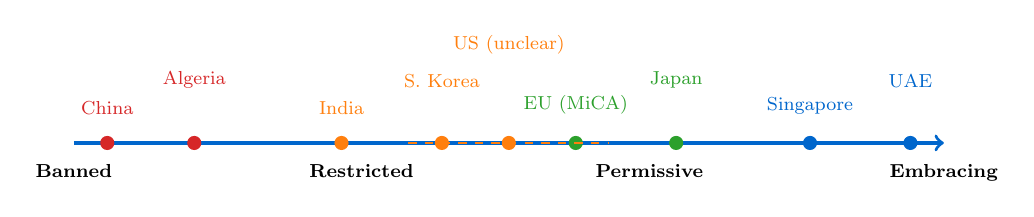
\begin{tikzpicture}[scale=0.85, transform shape]
% Spectrum line
\draw[very thick, ->, dfblue] (0,0) -- (13,0);
\node[below, font=\footnotesize] at (0,-0.2) {\textbf{Banned}};
\node[below, font=\footnotesize] at (4.3,-0.2) {\textbf{Restricted}};
\node[below, font=\footnotesize] at (8.6,-0.2) {\textbf{Permissive}};
\node[below, font=\footnotesize] at (13,-0.2) {\textbf{Embracing}};

% Country markers
\node[above, font=\footnotesize, text=dfred] at (0.5,0.3) {China};
\node[above, font=\footnotesize, text=dfred] at (1.8,0.7) {Algeria};

\node[above, font=\footnotesize, text=dforange] at (4,0.3) {India};
\node[above, font=\footnotesize, text=dforange] at (5.5,0.7) {S.~Korea};

\node[above, font=\footnotesize, text=dfgreen] at (7.5,0.3) {EU (MiCA)};
\node[above, font=\footnotesize, text=dfgreen] at (9,0.7) {Japan};

\node[above, font=\footnotesize, text=dfblue] at (11,0.3) {Singapore};
\node[above, font=\footnotesize, text=dfblue] at (12.5,0.7) {UAE};

% Dots on the line
\fill[dfred] (0.5,0) circle (3pt);
\fill[dfred] (1.8,0) circle (3pt);
\fill[dforange] (4,0) circle (3pt);
\fill[dforange] (5.5,0) circle (3pt);
\fill[dfgreen] (7.5,0) circle (3pt);
\fill[dfgreen] (9,0) circle (3pt);
\fill[dfblue] (11,0) circle (3pt);
\fill[dfblue] (12.5,0) circle (3pt);

% US special position
\node[above, font=\footnotesize, text=dforange] at (6.5,1.2) {US (unclear)};
\fill[dforange] (6.5,0) circle (3pt);
\draw[dashed, dforange] (5.0,0) -- (8.0,0);
\end{tikzpicture}
\end{center}

\vspace{3mm}
\begin{block}{Key Takeaway}
There is no single ``right'' approach. We will study the US (complex, fragmented), EU (comprehensive framework), and Asia (full spectrum from ban to innovation hub) in detail.
\end{block}

\vspace{2mm}
% [H31] Acknowledge US-heavy focus
\footnotesize \textbf{Note:} We spend more time on the US because it is the largest crypto market and its regulatory approach is the most complex. Other jurisdictions often follow or react to US decisions.
\end{frame}

% ==============================================================================
% SLIDE 8: How to Read a Regulatory Framework
% ==============================================================================
% [H28] Analytical framework slide
\begin{frame}{How to Read Any Regulatory Framework}
\textbf{When evaluating any country's approach to crypto regulation, ask these four questions:}
\vspace{5mm}

\begin{enumerate}
\item \textbf{Who regulates?}\\
Is there one regulator or many? Do they coordinate or compete?
\item \textbf{What is classified as what?}\\
Is a token a security, a commodity, a payment instrument, or something new?
\item \textbf{What is banned vs.\ permitted?}\\
Can you trade, issue tokens, run an exchange, offer DeFi services?
\item \textbf{How are consumers protected?}\\
Are there insurance schemes, disclosure requirements, or investor limits?
\end{enumerate}

\vspace{5mm}
\begin{block}{Use This Framework}
As we study each jurisdiction, apply these four questions. You will see how the same technology receives very different regulatory treatment depending on how each country answers them.
\end{block}
\end{frame}

% ==============================================================================
% SLIDE 9: The Regulatory Challenge
% ==============================================================================
\begin{frame}{The Regulatory Challenge}
\begin{columns}[T]
\begin{column}{0.48\textwidth}
\textbf{What regulators want:}
\begin{itemize}
\item Consumer protection
\item Market integrity
\item Financial stability
\item Anti-money laundering
\item Tax compliance
\item National security
\end{itemize}
\end{column}
\begin{column}{0.48\textwidth}
\textbf{What innovators want:}
\begin{itemize}
\item Permissionless access
\item Privacy
\item Speed to market
\item Global reach
\item Minimal compliance costs
\item Regulatory clarity
\end{itemize}
\end{column}
\end{columns}

\vspace{5mm}
\begin{center}
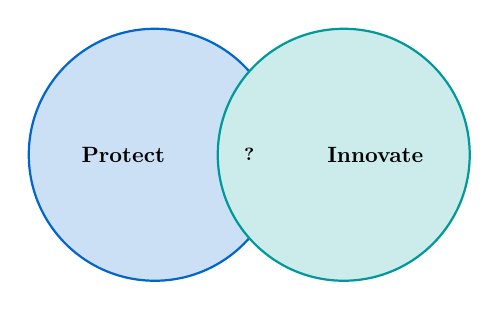
\begin{tikzpicture}[scale=0.8, transform shape]
\draw[thick, dfblue, fill=dfblue!20] (0,0) circle (2cm);
\draw[thick, dfteal, fill=dfteal!20] (3,0) circle (2cm);

\node at (-0.5,0) {\textbf{Protect}};
\node at (3.5,0) {\textbf{Innovate}};
\node at (1.5,0) {\footnotesize \textbf{?}};
\end{tikzpicture}
\end{center}
\end{frame}

% ==============================================================================
% SLIDE 10: US Regulatory Landscape -- The Big Two
% ==============================================================================
% [H24] Split into 2 slides: first the Big Two
\begin{frame}{United States: The Big Two Regulators}
\begin{center}
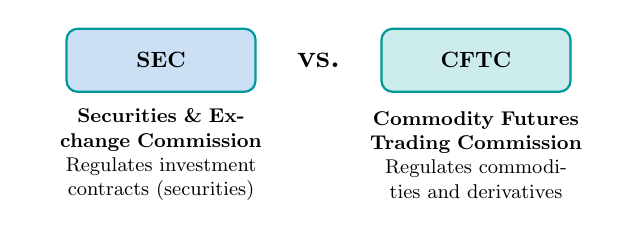
\begin{tikzpicture}[scale=0.8, transform shape]
% Two main agencies
\node (sec) [blockchain, minimum width=3cm, fill=dfblue!20] {\textbf{SEC}};
\node (cftc) [blockchain, right of=sec, node distance=5cm, minimum width=3cm, fill=dfteal!20] {\textbf{CFTC}};

% Labels
\node[below of=sec, node distance=1.5cm, font=\small, text width=4cm, align=center] {\textbf{Securities \& Exchange Commission}\\Regulates investment contracts (securities)};
\node[below of=cftc, node distance=1.5cm, font=\small, text width=4cm, align=center] {\textbf{Commodity Futures Trading Commission}\\Regulates commodities and derivatives};

% The question in the middle
\node[font=\Large] at (2.5,0) {\textbf{vs.}};
\end{tikzpicture}
\end{center}

\vspace{3mm}
\textbf{The central question in US crypto regulation:}
\begin{itemize}
\item Is a crypto token a \textbf{security} (regulated by the SEC)?
\item Or is it a \textbf{commodity} (regulated by the CFTC)?
\item Bitcoin and Ethereum: classified as \textbf{commodities}
\item Many other tokens: the SEC argues they are \textbf{securities}
\end{itemize}

\vspace{3mm}
\begin{alertblock}{Why This Matters}
Securities face strict rules: registration, disclosure documents, and restrictions on who can buy. Commodities face lighter regulation. The classification determines everything.
\end{alertblock}
\end{frame}

% ==============================================================================
% SLIDE 11: US Regulatory Landscape -- Supporting Agencies
% ==============================================================================
% [H24] Second part: supporting agencies
\begin{frame}{United States: Supporting Regulatory Agencies}
\begin{center}
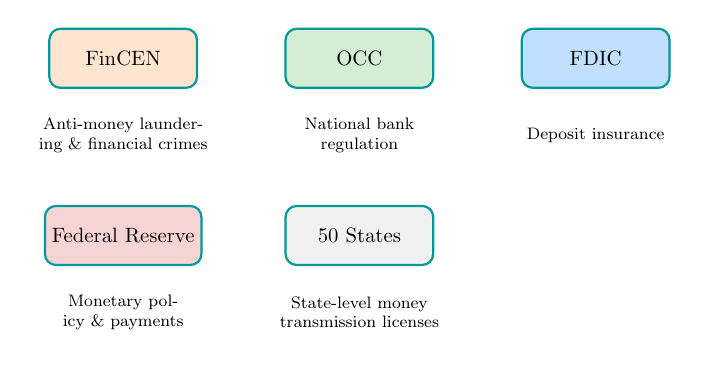
\begin{tikzpicture}[scale=0.75, transform shape]
% Supporting agencies
\node (fincen) [blockchain, minimum width=2.5cm, fill=dforange!20] {FinCEN};
\node (occ) [blockchain, right of=fincen, node distance=4cm, minimum width=2.5cm, fill=dfgreen!20] {OCC};
\node (fdic) [blockchain, right of=occ, node distance=4cm, minimum width=2.5cm, fill=dflightblue3] {FDIC};

% Labels
\node[below of=fincen, node distance=1.3cm, font=\footnotesize, text width=3cm, align=center] {Anti-money laundering \& financial crimes};
\node[below of=occ, node distance=1.3cm, font=\footnotesize, text width=3cm, align=center] {National bank regulation};
\node[below of=fdic, node distance=1.3cm, font=\footnotesize, text width=3cm, align=center] {Deposit insurance};

% Second row
\node (fed) [blockchain, below of=fincen, node distance=3cm, minimum width=2.5cm, fill=dfred!20] {Federal Reserve};
\node (state) [blockchain, below of=occ, node distance=3cm, minimum width=2.5cm, fill=lightgray] {50 States};

\node[below of=fed, node distance=1.3cm, font=\footnotesize, text width=3cm, align=center] {Monetary policy \& payments};
\node[below of=state, node distance=1.3cm, font=\footnotesize, text width=3cm, align=center] {State-level money transmission licenses};
\end{tikzpicture}
\end{center}

\vspace{3mm}
% [C7] Define "regulation by enforcement"
\begin{alertblock}{Key Issue: No Single Regulator}
No single agency is in charge of crypto. Jurisdictional conflicts between all these agencies create uncertainty and ``regulation by enforcement'' --- meaning regulators do not write new crypto-specific rules. Instead, they use existing laws and punish companies that break them. Think of it as: \textit{``we will tell you the rules by punishing those who break them.''}
\end{alertblock}
\end{frame}

% ==============================================================================
% SLIDE 12: The Howey Test
% ==============================================================================
\begin{frame}{US: The Howey Test}
\begin{columns}[T]
\begin{column}{0.55\textwidth}
\textbf{Is it a security?}\\
A token is a security if it involves:
\begin{enumerate}
\item \textbf{Investment of money}
\item \textbf{In a common enterprise}
\item \textbf{With expectation of profits}
\item \textbf{Derived from others' efforts}
\end{enumerate}

\vspace{3mm}
% [C8] Rental property analogy for Howey Test
\textbf{Analogy:} Think of buying a rental property managed by someone else:
\begin{enumerate}
\item You invest money (buying the property)
\item In a common enterprise (the building has multiple investors)
\item Expecting profits (rental income)
\item From others' efforts (the property manager does the work)
\end{enumerate}
$\rightarrow$ This is an ``investment contract'' = a security.
\end{column}
\begin{column}{0.42\textwidth}
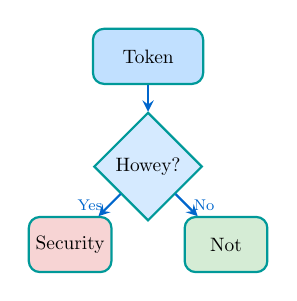
\begin{tikzpicture}[scale=0.7, transform shape]
% Decision tree
\node (start) [blockchain, minimum width=2cm] {Token};
\node (howey) [decision, below of=start, node distance=2cm, minimum width=1.5cm, minimum height=1.5cm] {Howey?};
\node (security) [blockchain, below left of=howey, node distance=2cm, fill=dfred!20, minimum width=1.5cm] {Security};
\node (commodity) [blockchain, below right of=howey, node distance=2cm, fill=dfgreen!20, minimum width=1.5cm] {Not};

\draw[arrow] (start) -- (howey);
\draw[arrow] (howey) -- node[left, font=\footnotesize] {Yes} (security);
\draw[arrow] (howey) -- node[right, font=\footnotesize] {No} (commodity);
\end{tikzpicture}

\vspace{3mm}
\textbf{SEC Position:}
\begin{itemize}
% [H17] Define ICO on first use
\item Most ICOs (Initial Coin Offerings --- a way for crypto projects to raise money by selling tokens directly to the public, similar to an IPO for stocks) were securities
\item Many tokens are securities
\item ETH and BTC are NOT securities
\end{itemize}
\end{column}
\end{columns}
\end{frame}

% ==============================================================================
% SLIDE 13: SEC vs CFTC Jurisdiction
% ==============================================================================
\begin{frame}{SEC vs.\ CFTC: Jurisdictional Divide}
\begin{center}
\renewcommand{\arraystretch}{1.3}
\begin{tabular}{|l|c|c|}
\hline
\textbf{Aspect} & \textbf{SEC} & \textbf{CFTC} \\
\hline
\textbf{Jurisdiction} & Securities & Commodities \\
\hline
\textbf{Key test} & Howey Test & Not a security \\
\hline
\textbf{Bitcoin} & Not a security & Commodity \\
\hline
\textbf{Ethereum} & Not a security (debated) & Commodity \\
\hline
% [H19] Define spot market
\textbf{Most altcoins} & Often securities & Spot market limited \\
\hline
\textbf{Stablecoins} & Unclear & Limited jurisdiction \\
\hline
\textbf{Exchanges} & Securities exchanges & Derivatives exchanges \\
\hline
\end{tabular}
\end{center}

\vspace{2mm}
% [H19] Spot market definition
\footnotesize \textbf{Term:} \textit{Spot market} = buying or selling for immediate delivery, as opposed to futures or options (which are contracts about future prices).

\vspace{2mm}
\normalsize
\begin{block}{The Gap}
Spot markets for crypto commodities (like Bitcoin) fall into a regulatory gap---CFTC has limited authority over spot trading, SEC claims none. Nobody is clearly in charge.
\end{block}
\end{frame}

% ==============================================================================
% SLIDE 14: FinCEN and AML Requirements
% ==============================================================================
\begin{frame}{FinCEN: AML/KYC Requirements}
% [H20] Define Bank Secrecy Act
\textbf{Financial Crimes Enforcement Network (FinCEN)}---enforces the Bank Secrecy Act (BSA, 1970), the foundation of US anti-money-laundering law. The BSA requires banks and financial businesses to report suspicious transactions to help detect money laundering.
\vspace{3mm}

\begin{columns}[T]
\begin{column}{0.48\textwidth}
\textbf{Who must register?}
\begin{itemize}
\item Crypto exchanges
\item Custodial wallet providers
\item Crypto ATM operators
\item Payment processors
% [H21] Define MSBs
\item As Money Services Businesses (MSBs --- businesses that transfer money, cash checks, or exchange currencies, including many crypto exchanges)
\end{itemize}
\end{column}
\begin{column}{0.48\textwidth}
\textbf{Requirements:}
\begin{itemize}
\item Customer identification (KYC)
\item Transaction monitoring
% [H22] Define SARs and CTRs
\item Suspicious Activity Reports (SARs --- filed when a business spots something unusual)
\item Currency Transaction Reports (CTRs --- required for transactions over \$10,000)
\item Record keeping (5 years)
\end{itemize}
\end{column}
\end{columns}

\vspace{3mm}
\begin{alertblock}{Key Point}
AML/KYC requirements apply regardless of whether tokens are securities or commodities. All crypto businesses touching fiat or custody must comply.
\end{alertblock}
\end{frame}

% ==============================================================================
% SLIDE 15: Checkpoint -- US Regulation So Far
% ==============================================================================
% [C9] Checkpoint/recap slide after dense US regulatory content
\begin{frame}{Checkpoint: US Regulation So Far}
\begin{block}{Let's Pause and Recap}
We have covered a lot of US-specific content. Here are the key points so far:
\end{block}

\vspace{3mm}
\begin{enumerate}
\item \textbf{Multiple regulators} --- The US has many agencies (SEC, CFTC, FinCEN, OCC, 50 states) with overlapping authority. No single ``crypto regulator'' exists.
\item \textbf{The key question:} Is a crypto token a \textbf{security} or a \textbf{commodity}? The answer determines which rules apply.
\item \textbf{The Howey Test} helps decide --- think of the rental property analogy: if you invest money, in a group venture, expecting profits from someone else's work, it is a security.
\item \textbf{AML/KYC applies to everyone} --- regardless of token classification, all crypto businesses must verify customer identities and report suspicious activity.
\item \textbf{``Regulation by enforcement''} --- the US currently makes rules by suing companies, rather than writing clear guidelines first.
\end{enumerate}

\vspace{3mm}
\textbf{Coming next:} Enforcement actions, state-level regulation, and how tokens can legally be issued.
\end{frame}

% ==============================================================================
% SLIDE 16: US Enforcement Actions
% ==============================================================================
\begin{frame}{US Enforcement Actions (2023--2024)}
\begin{center}
\renewcommand{\arraystretch}{1.3}
\begin{tabular}{|l|l|p{5cm}|}
\hline
\textbf{Target} & \textbf{Allegation} & \textbf{Status} \\
\hline
% [M1] Define "operating unregistered exchange"
Coinbase & Operating unregistered exchange (running a trading platform without SEC approval) & Ongoing litigation \\
\hline
Binance & Multiple securities violations & \$4.3B settlement \\
\hline
% [M2] Define "staking"
Kraken & Unregistered staking service (staking = locking up tokens to earn rewards) & \$30M settlement \\
\hline
Ripple (XRP) & Unregistered securities & Partial win for Ripple \\
\hline
Terraform & Securities fraud (UST) & Founders charged \\
\hline
\end{tabular}
\end{center}

\vspace{3mm}
\begin{alertblock}{Regulation by Enforcement}
The US lacks comprehensive crypto legislation. SEC and CFTC establish rules through lawsuits rather than clear guidelines --- companies often do not know they are breaking a rule until they are sued.
\end{alertblock}
\end{frame}

% ==============================================================================
% SLIDE 17: State-Level Regulation
% ==============================================================================
\begin{frame}{US State-Level Regulation: BitLicense Example}
% [H26] Add context about state regulation
\textbf{In the US, states can create their own financial regulations on top of federal rules.} New York's BitLicense (2015) was the first state-level crypto-specific license.
\vspace{3mm}

\begin{columns}[T]
\begin{column}{0.48\textwidth}
\textbf{Requirements:}
\begin{itemize}
\item Application fee + capital reserves
\item Comprehensive cybersecurity program
\item AML/KYC compliance plan
\item Consumer protection measures
\item Books and records requirements
\item Regular examinations
\end{itemize}
\end{column}
\begin{column}{0.48\textwidth}
\textbf{Impact:}
\begin{itemize}
\item Many companies exit NY market
\item High compliance costs
\item Lengthy approval process
\item But: regulatory clarity
\item Other states: Wyoming (friendly), Texas (mixed)
\end{itemize}
\end{column}
\end{columns}

\vspace{3mm}
% [C10] 50-state analogy
\begin{block}{The 50-State Problem}
Each US state has different money transmission rules. Operating nationally requires up to 50 separate licenses.

\textbf{Analogy:} Imagine opening a restaurant --- you would need a different license in every state, plus a federal one. Now imagine doing that in 50 states simultaneously. That is the challenge facing crypto companies in the US.
\end{block}
\end{frame}

% ==============================================================================
% SLIDE 18: Securities Exemptions (Simplified)
% ==============================================================================
% [H23] Simplified from graduate-level to plain English
\begin{frame}{US: If Your Token Is a Security, What Are Your Options?}
\textbf{If the Howey Test says your token is a security, you have two main paths:}
\vspace{5mm}

\begin{center}
\renewcommand{\arraystretch}{1.6}
\begin{tabular}{|l|p{9cm}|}
\hline
\textbf{Path} & \textbf{What It Means in Plain English} \\
\hline
% [M3][M4][M5] Define private placement, general solicitation, accredited investor
\textbf{Reg D} (Private Placement) & Sell only to \textbf{accredited investors} --- people wealthy enough (income over \$200K/year or net worth over \$1M) or experienced enough that regulators assume they can handle risky investments. No public advertising allowed in most cases. \\
\hline
\textbf{Reg A+} (Mini-IPO) & A simplified version of a full public offering. Less paperwork than a traditional IPO, and \textbf{anyone} can invest (with limits). Maximum raise: \$75M. \\
\hline
\end{tabular}
\end{center}

\vspace{3mm}
\footnotesize
\textbf{Other options:} Reg S (sell only outside the US), Reg CF (crowdfunding up to \$5M through registered portals). All exemptions have strict requirements --- violations trigger enforcement.

\vspace{3mm}
\normalsize
% [H18] Define prospectus and qualified investors
\begin{block}{Key Terms}
\textbf{Prospectus} = detailed document explaining the investment and its risks (like a product manual for investors). \textbf{Accredited/qualified investor} = someone wealthy or experienced enough that regulators assume they can handle risky investments.
\end{block}
\end{frame}

% ==============================================================================
% SLIDE 19: Transition to EU
% ==============================================================================
% [M14] Bridge sentence from US to EU
\begin{frame}{From US Fragmentation to EU Harmonization}
\begin{block}{Change of Approach}
We have just seen the US approach: multiple agencies, overlapping authority, regulation by enforcement, and significant uncertainty. Now let's see a very different model.
\end{block}

\vspace{5mm}
\begin{center}
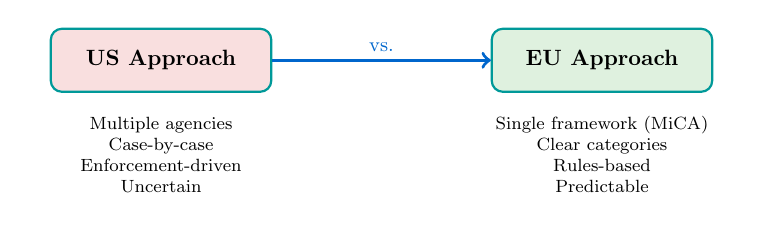
\begin{tikzpicture}[scale=0.8, transform shape]
\node (us) [blockchain, minimum width=3.5cm, fill=dfred!15] {\textbf{US Approach}};
\node (eu) [blockchain, right of=us, node distance=7cm, minimum width=3.5cm, fill=dfgreen!15] {\textbf{EU Approach}};

\draw[->, very thick, dfblue] (us) -- node[above, font=\small] {vs.} (eu);

\node[below of=us, node distance=1.5cm, font=\footnotesize, text width=4cm, align=center] {Multiple agencies\\Case-by-case\\Enforcement-driven\\Uncertain};
\node[below of=eu, node distance=1.5cm, font=\footnotesize, text width=4cm, align=center] {Single framework (MiCA)\\Clear categories\\Rules-based\\Predictable};
\end{tikzpicture}
\end{center}

\vspace{5mm}
\textbf{The EU asked:} ``What if we wrote clear rules \textit{before} problems happen, instead of suing companies after the fact?''
\end{frame}

% ==============================================================================
% SLIDE 20: EU MiCA Framework
% ==============================================================================
\begin{frame}{European Union: MiCA Framework}
\begin{columns}[T]
\begin{column}{0.55\textwidth}
\textbf{Markets in Crypto-Assets (MiCA):}
\begin{itemize}
\item First comprehensive crypto regulation
\item Effective 2024--2025
\item Harmonized across 27 countries
\item Clear licensing requirements
\end{itemize}

\vspace{3mm}
\textbf{Key Provisions:}
\begin{enumerate}
\item Crypto-Asset Service Providers (CASPs) licensed
\item Stablecoin issuers must hold reserves
\item Whitepaper requirements for token issuance
\item Consumer protection rules
\item Market manipulation prohibited
\end{enumerate}
\end{column}
\begin{column}{0.42\textwidth}
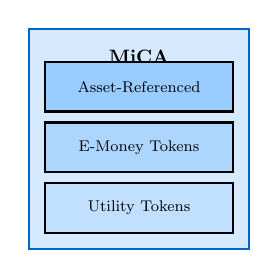
\begin{tikzpicture}[scale=0.7, transform shape]
% MiCA structure
\draw[thick, dfblue, fill=dflightblue4] (0,0) rectangle (4,4);
\node at (2,3.5) {\textbf{MiCA}};

\draw[thick, fill=dflightblue3] (0.3,0.3) rectangle (3.7,1.2);
\node[font=\footnotesize] at (2,0.75) {Utility Tokens};

\draw[thick, fill=dflightblue2] (0.3,1.4) rectangle (3.7,2.3);
\node[font=\footnotesize] at (2,1.85) {E-Money Tokens};

\draw[thick, fill=dflightblue] (0.3,2.5) rectangle (3.7,3.4);
\node[font=\footnotesize] at (2,2.95) {Asset-Referenced};
\end{tikzpicture}

\vspace{3mm}
\footnotesize
\textbf{Not covered:}\\
DeFi, NFTs (mostly), CBDCs
\end{column}
\end{columns}
\end{frame}

% ==============================================================================
% SLIDE 21: MiCA Token Categories
% ==============================================================================
\begin{frame}{MiCA: Token Categories}
\begin{center}
\renewcommand{\arraystretch}{1.4}
\footnotesize
\begin{tabular}{|l|p{4cm}|p{5cm}|}
\hline
\textbf{Category} & \textbf{Definition} & \textbf{Requirements} \\
\hline
\textbf{Utility Tokens} & Provide access to goods/services on a platform & Whitepaper, fair marketing, basic disclosure \\
\hline
\textbf{Asset-Referenced Tokens (ARTs)} & Value references multiple assets, commodities, or currencies & Authorization, reserve requirements, no interest payments \\
\hline
\textbf{E-Money Tokens (EMTs)} & Pegged 1:1 to single fiat currency & E-money institution license, 1:1 redemption, segregated reserves \\
\hline
\textbf{Other crypto-assets} & BTC, ETH, and similar & Lighter touch, no issuer requirements \\
\hline
\end{tabular}
\end{center}

\vspace{3mm}
\begin{block}{Key Distinction}
MiCA creates clear categories with proportionate requirements---unlike the US binary security/commodity debate.
\end{block}
\end{frame}

% ==============================================================================
% SLIDE 22: MiCA Stablecoin Rules
% ==============================================================================
\begin{frame}{MiCA: Stablecoin Rules}
\begin{columns}[T]
\begin{column}{0.48\textwidth}
\textbf{Asset-Referenced Tokens (ARTs):}
\begin{itemize}
\item Backed by multiple assets
\item Issuer must be authorized
\item Reserve requirements
\item No interest payments
\item If ``significant'': stricter rules
\end{itemize}

\vspace{3mm}
\textbf{E-Money Tokens (EMTs):}
\begin{itemize}
\item Single fiat currency reference
\item Must be e-money institution
\item 1:1 redemption rights
\item Segregated reserves
\end{itemize}
\end{column}
\begin{column}{0.48\textwidth}
\begin{alertblock}{Significance Thresholds}
``Significant'' ART/EMT if:
\begin{itemize}
\item 10M+ holders
% [L3] Add "euros" after EUR
\item 5 billion euros+ market cap
\item 2.5M+ daily transactions
\item 500 million euros+ daily value
\end{itemize}
Higher capital, stricter oversight.
\end{alertblock}

\vspace{3mm}
\textbf{Impact on USDT/USDC:}\\
Must comply or delist from EU exchanges.
\end{column}
\end{columns}
\end{frame}

% ==============================================================================
% SLIDE 23: MiCA Service Provider Rules
% ==============================================================================
\begin{frame}{MiCA: Crypto-Asset Service Providers (CASPs)}
\textbf{Services requiring CASP license:}
\vspace{2mm}

\begin{multicols}{2}
\begin{itemize}
\item Custody and administration
\item Operating a trading platform
\item Exchange of crypto for fiat
\item Exchange of crypto for crypto
\item Execution of orders
\item Placing of crypto-assets
\item Transfer services
\item Advice on crypto-assets
\item Portfolio management
\end{itemize}
\end{multicols}

\vspace{3mm}
\textbf{CASP Requirements:}
\begin{itemize}
% [M6] Define "passportable"
\item Authorization in one EU member state (passportable --- meaning the license is usable across all EU countries)
\item Minimum capital requirements
\item Governance and organizational requirements
\item Safeguarding of client assets
\item Complaints handling procedures
\end{itemize}

\vspace{3mm}
\begin{block}{Passporting}
Once licensed in one EU country, CASPs can operate across all 27 member states --- a major advantage over the US 50-state problem.
\end{block}
\end{frame}

% ==============================================================================
% SLIDE 24: Asia Diverse Approaches
% ==============================================================================
\begin{frame}{Asia: Diverse Regulatory Approaches}
\begin{center}
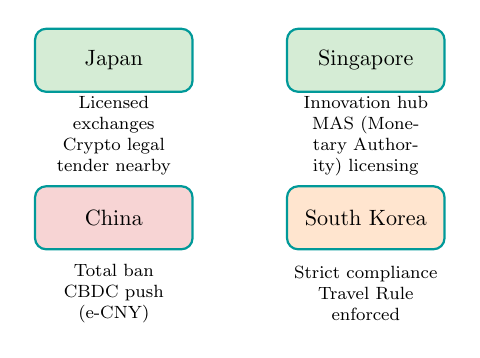
\begin{tikzpicture}[scale=0.8, transform shape]
% Map representation
\node (japan) [blockchain, minimum width=2.5cm, fill=dfgreen!20] {Japan};
\node (singapore) [blockchain, right of=japan, node distance=4cm, minimum width=2.5cm, fill=dfgreen!20] {Singapore};
\node (china) [blockchain, below of=japan, node distance=2.5cm, minimum width=2.5cm, fill=dfred!20] {China};
\node (korea) [blockchain, below of=singapore, node distance=2.5cm, minimum width=2.5cm, fill=dforange!20] {South Korea};

% Labels
\node[below of=japan, node distance=1.2cm, font=\footnotesize, text width=2.5cm, align=center] {Licensed exchanges\\Crypto legal tender nearby};
% [L1] Expand MAS before use
\node[below of=singapore, node distance=1.2cm, font=\footnotesize, text width=2.5cm, align=center] {Innovation hub\\MAS (Monetary Authority) licensing};
\node[below of=china, node distance=1.2cm, font=\footnotesize, text width=2.5cm, align=center] {Total ban\\CBDC push (e-CNY)};
% [C10] Travel Rule analogy
\node[below of=korea, node distance=1.2cm, font=\footnotesize, text width=2.5cm, align=center] {Strict compliance\\Travel Rule enforced};
\end{tikzpicture}
\end{center}

\vspace{3mm}
% [C10] Travel Rule analogy
\textbf{Analogy --- Travel Rule:} Like registered mail --- the sender and receiver must be identified for transfers above a certain amount. South Korea enforces this strictly.

\vspace{2mm}
\textbf{Key insight:} Asia demonstrates the full spectrum from complete ban (China) to innovation hub (Singapore).
\end{frame}

% ==============================================================================
% SLIDE 25: Singapore MAS
% ==============================================================================
\begin{frame}{Singapore: Innovation Hub with Clear Rules}
% [L1] MAS already expanded in previous slide
\textbf{Monetary Authority of Singapore (MAS) Approach}
\vspace{3mm}

\begin{columns}[T]
\begin{column}{0.48\textwidth}
\textbf{Regulatory Framework:}
\begin{itemize}
\item Payment Services Act (PSA) 2019
\item Digital Payment Token (DPT) license
\item Clear licensing categories
\item Risk-based supervision
\item Regulatory sandbox available
\end{itemize}
\end{column}
\begin{column}{0.48\textwidth}
\textbf{Requirements:}
\begin{itemize}
% [M7] Expand CFT
\item AML/CFT (Combating the Financing of Terrorism) compliance
\item Technology risk management
\item User protection measures
\item Capital requirements
% [L4] Explain "fit and proper"
\item Fit and proper management (meaning directors and key staff must demonstrate honesty, competence, and financial soundness)
\end{itemize}
\end{column}
\end{columns}

\vspace{5mm}
\begin{block}{Singapore's Strategy}
Attract compliant crypto businesses with clear rules, strict enforcement, and innovation support---while banning retail crypto advertising.
\end{block}
\end{frame}

% ==============================================================================
% SLIDE 26: China Complete Ban
% ==============================================================================
\begin{frame}{China: Complete Ban + CBDC}
\begin{columns}[T]
\begin{column}{0.48\textwidth}
\textbf{What's Banned:}
\begin{itemize}
\item Cryptocurrency trading
\item Crypto mining (since 2021)
\item ICOs (token fundraising)
\item Crypto exchanges
\item Providing crypto services
\end{itemize}

\vspace{3mm}
\textbf{Penalties:}
\begin{itemize}
\item Criminal prosecution possible
\item Businesses shut down
\item Mining operations seized
\end{itemize}
\end{column}
\begin{column}{0.48\textwidth}
\textbf{Digital Yuan (e-CNY):}
\begin{itemize}
\item Central Bank Digital Currency
\item Controlled by PBoC
\item Two-tier distribution
\item Programmable money
\item Pilot programs in major cities
\end{itemize}

\vspace{3mm}
\begin{alertblock}{The Strategy}
Ban decentralized crypto, promote centralized CBDC. Maximum control, full surveillance.
\end{alertblock}
\end{column}
\end{columns}
\end{frame}

% ==============================================================================
% SLIDE 27: Japan and South Korea
% ==============================================================================
\begin{frame}{Japan and South Korea: Regulated Markets}
\begin{columns}[T]
\begin{column}{0.48\textwidth}
\textbf{Japan (FSA):}
\begin{itemize}
\item First major country to license exchanges (2017)
\item Crypto as ``payment method''
\item Strict exchange requirements
% [M9] Define cold wallet
\item Cold wallet mandate (cold wallet = offline storage, not connected to the internet, harder for hackers to reach)
% [M8] Expand JVCEA
\item Self-regulatory organization: JVCEA (Japan Virtual and Crypto Assets Exchange Association)
\item Response to Mt.\ Gox collapse
\end{itemize}
\end{column}
\begin{column}{0.48\textwidth}
\textbf{South Korea:}
\begin{itemize}
% [M19] Explain real-name system
\item Real-name trading accounts (every crypto trader must link their exchange account to a bank account in their real, verified name --- no anonymous trading)
\item Bank partnerships required
\item Strict Travel Rule enforcement
\item Tax on crypto gains
\item Major exchange oversight
\item High retail participation
\end{itemize}
\end{column}
\end{columns}

\vspace{3mm}
\begin{block}{Common Thread}
Both markets experienced major hacks/scandals that drove stricter regulation. Compliance-focused but open to innovation.
\end{block}
\end{frame}

% ==============================================================================
% SLIDE 28: Regulatory Comparison Matrix
% ==============================================================================
\begin{frame}{Regulatory Comparison Matrix}
\begin{center}
\renewcommand{\arraystretch}{1.2}
\footnotesize
\begin{tabular}{|l|c|c|c|c|}
\hline
\textbf{Aspect} & \textbf{US} & \textbf{EU (MiCA)} & \textbf{Singapore} & \textbf{China} \\
\hline
Crypto trading & Varies & Licensed & Licensed & \textcolor{dfred}{Banned} \\
\hline
Token issuance & Case-by-case & Whitepaper & Licensed & \textcolor{dfred}{Banned} \\
\hline
Stablecoins & Unclear & Regulated & Licensed & \textcolor{dfred}{Banned} \\
\hline
DeFi & Unclear & Unclear & Evolving & \textcolor{dfred}{Banned} \\
\hline
NFTs & Unclear & Mostly exempt & Evolving & Gray area \\
\hline
CBDC & Researching & Exploring & Exploring & \textcolor{dfgreen}{Live} \\
\hline
Clarity & \textcolor{dfred}{Low} & \textcolor{dfgreen}{High} & \textcolor{dforange}{Medium} & \textcolor{dfgreen}{High (ban)} \\
\hline
\end{tabular}
\end{center}

\vspace{3mm}
\begin{block}{Key Insight}
Regulatory arbitrage is real. Projects choose jurisdictions strategically. Clear rules (even strict ones) often preferred over uncertainty.
\end{block}
\end{frame}

% ==============================================================================
% SLIDE 29: The Travel Rule
% ==============================================================================
\begin{frame}{The Travel Rule (FATF Recommendation 16)}
\begin{columns}[T]
\begin{column}{0.55\textwidth}
\textbf{What is it?}\\
% [C10] Travel Rule analogy repeated with detail
FATF requirement: Virtual Asset Service Providers (VASPs) must share sender/receiver information for transfers above thresholds. \textbf{Analogy:} Like registered mail --- both sender and receiver must be identified.

\vspace{3mm}
\textbf{Information Required:}
\begin{itemize}
\item Sender name
\item Sender account number
\item Sender address or ID
\item Beneficiary name
\item Beneficiary account number
\end{itemize}

\vspace{3mm}
\textbf{Thresholds:}
\begin{itemize}
\item US: \$3,000+
\item EU: 0 euros (all transfers!)
\item FATF guidance: \$1,000
\end{itemize}
\end{column}
\begin{column}{0.42\textwidth}
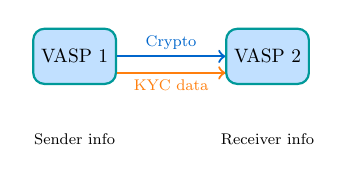
\begin{tikzpicture}[scale=0.7, transform shape, node distance=2cm]
% Travel rule flow
\node (vasp1) [blockchain, minimum width=1.5cm] {VASP 1};
\node (vasp2) [blockchain, right of=vasp1, node distance=3.5cm, minimum width=1.5cm] {VASP 2};

\draw[->, thick, dfblue] (vasp1) -- node[above, font=\footnotesize] {Crypto} (vasp2);
\draw[->, thick, dforange] ([yshift=-3mm]vasp1.east) -- node[below, font=\footnotesize] {KYC data} ([yshift=-3mm]vasp2.west);

\node[below of=vasp1, node distance=1.5cm, font=\footnotesize] {Sender info};
\node[below of=vasp2, node distance=1.5cm, font=\footnotesize] {Receiver info};
\end{tikzpicture}

\vspace{5mm}
\begin{alertblock}{DeFi Challenge}
How do you apply Travel Rule to non-custodial wallets and DEXs with no central operator?
\end{alertblock}
\end{column}
\end{columns}
\end{frame}

% ==============================================================================
% SLIDE 30: DeFi Regulatory Challenges
% ==============================================================================
\begin{frame}{DeFi Regulatory Challenges}
\begin{columns}[T]
\begin{column}{0.48\textwidth}
\textbf{The Fundamental Problem:}
\begin{itemize}
\item Who is the ``operator''?
\item Where is it located?
\item Who do you regulate?
\item How do you enforce?
\end{itemize}

\vspace{3mm}
\textbf{Potential Targets:}
\begin{itemize}
\item Frontend interfaces
\item Token holders with governance power
\item Core developers
\item Infrastructure providers
\end{itemize}
\end{column}
\begin{column}{0.48\textwidth}
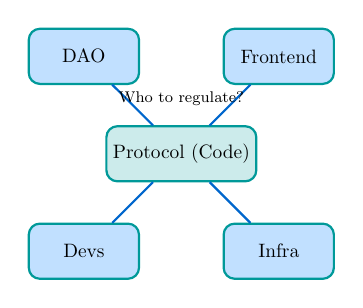
\begin{tikzpicture}[scale=0.7, transform shape]
% DeFi structure
\node (protocol) [blockchain, minimum width=2.5cm, fill=dfteal!20] {Protocol (Code)};
\node (governance) [blockchain, above left of=protocol, node distance=2.5cm, minimum width=2cm] {DAO};
\node (frontend) [blockchain, above right of=protocol, node distance=2.5cm, minimum width=2cm] {Frontend};
\node (devs) [blockchain, below left of=protocol, node distance=2.5cm, minimum width=2cm] {Devs};
\node (infra) [blockchain, below right of=protocol, node distance=2.5cm, minimum width=2cm] {Infra};

\draw[thick, dfblue] (governance) -- (protocol);
\draw[thick, dfblue] (frontend) -- (protocol);
\draw[thick, dfblue] (devs) -- (protocol);
\draw[thick, dfblue] (infra) -- (protocol);

\node[above of=protocol, node distance=1cm, font=\footnotesize] {Who to regulate?};
\end{tikzpicture}
\end{column}
\end{columns}

\vspace{3mm}
% [L2] Explain "chokepoints" in plain English
\begin{block}{Emerging Approach}
Target the \textbf{chokepoints} (the few places where regulators can exert control): fiat on/off ramps (where crypto meets traditional money), centralized frontends (the websites users interact with), and infrastructure providers (the companies running the servers).
\end{block}
\end{frame}

% ==============================================================================
% SLIDE 31: Regulatory Sandbox Concept
% ==============================================================================
\begin{frame}{Regulatory Sandboxes}
\textbf{A controlled environment for innovation under regulatory supervision}
\vspace{3mm}

\begin{columns}[T]
\begin{column}{0.48\textwidth}
\textbf{How Sandboxes Work:}
\begin{enumerate}
\item Company applies with innovative product
\item Regulator grants limited authorization
\item Testing with real users, limited scale
\item Relaxed rules during trial period
\item Evaluation and exit to full compliance
\end{enumerate}
\end{column}
\begin{column}{0.48\textwidth}
\textbf{Countries with Crypto Sandboxes:}
\begin{itemize}
\item UK (FCA)
\item Singapore (MAS)
\item Switzerland (FINMA)
\item UAE (ADGM, DIFC)
\item Bermuda
\item Australia (ASIC)
\end{itemize}
\end{column}
\end{columns}

\vspace{5mm}
\begin{block}{Benefits}
Regulators learn about new technologies. Innovators get clarity. Both sides reduce risk.
\end{block}
\end{frame}

% ==============================================================================
% SLIDE 32: Case Study - Tornado Cash
% ==============================================================================
\begin{frame}{Case Study: Tornado Cash Sanctions}
\begin{columns}[T]
\begin{column}{0.55\textwidth}
\textbf{What Happened (Aug 2022):}
\begin{itemize}
% [M10] Expand and explain OFAC
\item US Treasury sanctioned Tornado Cash via OFAC (Office of Foreign Assets Control --- the agency that enforces economic sanctions)
\item Smart contract addresses added to sanctions list
\item Developer arrested in Netherlands
\item First time: CODE itself sanctioned
\end{itemize}

\vspace{3mm}
\textbf{Consequences:}
\begin{itemize}
\item GitHub removed repository
\item Circle froze USDC in flagged addresses
\item Exchanges blocked deposits
% [M11] Define Alchemy/Infura/RPC
\item Alchemy and Infura (companies providing blockchain access services) blocked RPC access (RPC = the technical connection applications use to communicate with the blockchain)
\end{itemize}
\end{column}
\begin{column}{0.42\textwidth}
\begin{alertblock}{Legal Questions}
\begin{itemize}
\item Can you sanction open-source code?
\item Is running a mixer illegal?
\item What about privacy rights?
% [H29] Explain First Amendment
\item First Amendment implications? (The First Amendment to the US Constitution protects free speech --- some argue that code is speech)
\end{itemize}
\end{alertblock}

\vspace{3mm}
\textbf{Outcome:}\\
Court ruled some sanctions overreach (2024). Case ongoing.
\end{column}
\end{columns}
\end{frame}

% ==============================================================================
% SLIDE 33: Case Study - Ripple XRP
% ==============================================================================
\begin{frame}{Case Study: SEC vs.\ Ripple (XRP)}
\textbf{The landmark case defining token classification}
\vspace{3mm}

\begin{columns}[T]
\begin{column}{0.48\textwidth}
\textbf{SEC's Position:}
\begin{itemize}
\item XRP is a security
\item Ripple raised \$1.3B through unregistered sales
\item Investors expected profits from Ripple's efforts
\item Howey Test clearly applies
\end{itemize}

\vspace{3mm}
\textbf{Timeline:}
\begin{itemize}
\item Dec 2020: SEC files lawsuit
\item July 2023: Summary judgment
\item 2024: Ongoing appeals
\end{itemize}
\end{column}
\begin{column}{0.48\textwidth}
\textbf{July 2023 Ruling:}
\begin{itemize}
\item \textcolor{dfred}{Institutional sales = Securities}
\item \textcolor{dfgreen}{Exchange sales = NOT securities}
\item Programmatic sales to anonymous buyers don't meet Howey
\end{itemize}

\vspace{3mm}
\begin{alertblock}{Implications}
Secondary market trading may not create securities liability. Context matters more than the token itself.
\end{alertblock}
\end{column}
\end{columns}
\end{frame}

% ==============================================================================
% SLIDE 34: Case Study - Terra/Luna Collapse
% ==============================================================================
\begin{frame}{Case Study: Terra/Luna Regulatory Aftermath}
\textbf{How regulators respond to a \$40B+ collapse}
\vspace{3mm}

% [H25] Back-reference to T4.3
\textit{Recall from Day 4 (Topic 4.3): We studied how algorithmic stablecoins like UST tried to maintain their dollar peg through automatic mechanisms. Here is what happened when that mechanism failed:}
\vspace{2mm}

\begin{columns}[T]
\begin{column}{0.48\textwidth}
\textbf{What Happened (May 2022):}
\begin{itemize}
\item UST stablecoin de-pegged
\item Algorithmic mechanism failed
\item LUNA dropped 99.99\%
\item \$40B+ market cap destroyed
\item Cascading failures across DeFi
\end{itemize}
\end{column}
\begin{column}{0.48\textwidth}
\textbf{Regulatory Response:}
\begin{itemize}
\item SEC: Securities fraud charges
\item South Korea: Arrest warrants
\item Do Kwon: Arrested in Montenegro
\item MiCA: Influenced stablecoin rules
\item Accelerated global regulation
\end{itemize}
\end{column}
\end{columns}

\vspace{3mm}
\begin{block}{Lesson}
Systemic failures trigger regulatory action. Terra accelerated stablecoin regulation globally, especially in EU (MiCA) and proposed US legislation.
\end{block}
\end{frame}

% ==============================================================================
% SLIDE 35: Case Study - FTX and Exchange Regulation
% ==============================================================================
\begin{frame}{Case Study: FTX Collapse and Exchange Oversight}
\textbf{The case that changed crypto regulation permanently}
\vspace{3mm}

\begin{columns}[T]
\begin{column}{0.48\textwidth}
\textbf{What Failed (Nov 2022):}
\begin{itemize}
% [M18] Add context for Alameda Research
\item Customer funds mixed with Alameda Research (the trading firm secretly run by FTX's founder, Sam Bankman-Fried)
\item No segregation of assets
\item Fraudulent accounting
\item \$8B+ customer funds missing
\item Major contagion effects
\end{itemize}
\end{column}
\begin{column}{0.48\textwidth}
\textbf{Regulatory Implications:}
\begin{itemize}
\item Proof of reserves demanded
\item Customer asset segregation
\item Enhanced disclosure requirements
\item Congressional hearings
\item Accelerated legislation efforts
\end{itemize}
\end{column}
\end{columns}

\vspace{3mm}
\begin{alertblock}{Key Takeaway}
FTX showed that offshore exchanges serving US customers remain enforcement targets. ``Regulatory arbitrage'' has limits when fraud is involved.
\end{alertblock}
\end{frame}

% ==============================================================================
% SLIDE 36: Case Study Synthesis
% ==============================================================================
% [M12] Comparison table synthesizing all four case studies
\begin{frame}{Case Study Synthesis: What Do These Cases Teach Us?}
\begin{center}
\renewcommand{\arraystretch}{1.3}
\footnotesize
\begin{tabular}{|l|l|l|l|}
\hline
\textbf{Case} & \textbf{Core Issue} & \textbf{Regulatory Response} & \textbf{Lesson} \\
\hline
Tornado Cash & Can code be sanctioned? & OFAC sanctions on smart contracts & Privacy vs.\ compliance tension \\
\hline
Ripple (XRP) & Is XRP a security? & SEC lawsuit, partial loss & Context matters, not just token \\
\hline
Terra/Luna & Algorithmic stablecoin failure & Global stablecoin rules (MiCA) & Systemic risk drives regulation \\
\hline
FTX & Exchange fraud & Proof of reserves, segregation & Offshore is not beyond reach \\
\hline
\end{tabular}
\end{center}

\vspace{5mm}
\begin{block}{Pattern}
Every major crypto disaster follows the same cycle: \textbf{Innovation $\rightarrow$ Growth $\rightarrow$ Failure $\rightarrow$ Public outrage $\rightarrow$ New regulation.} Understanding this cycle helps you predict what regulators will do next.
\end{block}
\end{frame}

% ==============================================================================
% SLIDE 37: Discussion - Regulatory Philosophy
% ==============================================================================
\begin{frame}{Discussion: Regulatory Philosophy}
\begin{columns}[T]
\begin{column}{0.48\textwidth}
\textbf{Argument for Strict Regulation:}
\begin{itemize}
\item Protect consumers from fraud
\item Prevent money laundering
\item Ensure financial stability
% [H30] Define TradFi
\item Level playing field with TradFi (Traditional Finance --- crypto community's term for conventional banks, stock exchanges, and financial institutions)
\item Accountability for failures
\end{itemize}
\end{column}
\begin{column}{0.48\textwidth}
\textbf{Argument for Light Touch:}
\begin{itemize}
\item Enable innovation
\item Avoid regulatory arbitrage
% [H29] Already explained above; keep consistent
\item Code is speech (First Amendment --- US constitutional protection of free expression)
\item Self-sovereignty rights
\item Over-regulation pushes activity offshore
\end{itemize}
\end{column}
\end{columns}

\vspace{3mm}
% [H31] Acknowledge US-heavy focus
\footnotesize \textbf{Note:} We have spent more time on the US because it is the largest crypto market and its regulatory approach is the most complex. Other jurisdictions often follow or react to US decisions.

\vspace{2mm}
\normalsize
\begin{block}{Discussion Questions}
\begin{itemize}
\item Should DeFi protocols be regulated like banks?
\item Is ``code is law'' compatible with rule of law?
\item What is the right balance for stablecoins?
\item Where would you launch a crypto startup, and why?
\end{itemize}
\end{block}
\end{frame}

% ==============================================================================
% SLIDE 38: Application - Regulatory Strategy
% ==============================================================================
% [L5] Strategy slide kept in position (near end is appropriate for application)
\begin{frame}{Application: Building a Regulatory Strategy}
\textbf{For any digital finance project, consider:}
\vspace{3mm}

\begin{enumerate}
\item \textbf{Token Classification:} Is your token a security, commodity, utility, or payment token?
\item \textbf{Jurisdiction Selection:} Where will you incorporate, operate, and serve users?
\item \textbf{License Requirements:} What licenses needed in each target market?
\item \textbf{AML/KYC Design:} How will you comply with identity and monitoring rules?
\item \textbf{Consumer Protection:} What disclosures, safeguards, and recourse mechanisms?
\item \textbf{Future-Proofing:} How might regulations evolve? Build flexibility.
\end{enumerate}

\vspace{5mm}
\begin{alertblock}{Reality Check}
Compliance is expensive. Budget 15--30\% of early-stage costs for legal and regulatory work.
\end{alertblock}
\end{frame}

% ==============================================================================
% SLIDE 39: Executive Summary
% ==============================================================================
\begin{frame}{Executive Summary}
\begin{block}{Key Takeaways}
\begin{enumerate}
\item \textbf{US:} Fragmented regulation, enforcement-driven approach, Howey Test determines security status
\item \textbf{EU (MiCA):} First comprehensive framework, clear categories, passportable licenses
\item \textbf{Asia:} Full spectrum from ban (China) to innovation hub (Singapore)
\item \textbf{Global trend:} Moving toward regulation, focus on stablecoins and consumer protection
\item \textbf{DeFi:} Fundamental challenge---who/what to regulate when there is no central operator
\item \textbf{Strategy:} Regulatory clarity (even if strict) often preferred over uncertainty
\end{enumerate}
\end{block}

\vspace{3mm}
\textbf{The Bottom Line:} Regulation is not optional. Understanding regulatory logic helps you build compliant products and predict market evolution.
\end{frame}

% ==============================================================================
% SLIDE 40: Concept Map
% ==============================================================================
\begin{frame}{Concept Map: Regulatory Landscape}
\begin{center}
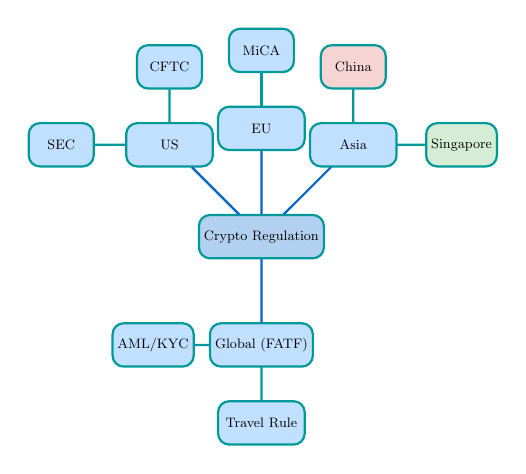
\begin{tikzpicture}[scale=0.55, transform shape,
    node distance=1.8cm,
    every node/.style={font=\small}]

% Central node
\node (reg) [blockchain, minimum width=2.5cm, fill=dfblue!30] {Crypto Regulation};

% First level
\node (us) [blockchain, above left of=reg, node distance=3cm, minimum width=2cm] {US};
\node (eu) [blockchain, above of=reg, node distance=2.5cm, minimum width=2cm] {EU};
\node (asia) [blockchain, above right of=reg, node distance=3cm, minimum width=2cm] {Asia};
\node (global) [blockchain, below of=reg, node distance=2.5cm, minimum width=2cm] {Global (FATF)};

% Second level - US
\node (sec) [blockchain, left of=us, node distance=2.5cm, minimum width=1.5cm, fill=dflightblue3] {SEC};
\node (cftc) [blockchain, above of=us, node distance=1.8cm, minimum width=1.5cm, fill=dflightblue3] {CFTC};

% Second level - EU
\node (mica) [blockchain, above of=eu, node distance=1.8cm, minimum width=1.5cm, fill=dflightblue3] {MiCA};

% Second level - Asia
\node (sg) [blockchain, right of=asia, node distance=2.5cm, minimum width=1.5cm, fill=dfgreen!20] {Singapore};
\node (cn) [blockchain, above of=asia, node distance=1.8cm, minimum width=1.5cm, fill=dfred!20] {China};

% Second level - Global
\node (travel) [blockchain, below of=global, node distance=1.8cm, minimum width=2cm, fill=dflightblue3] {Travel Rule};
\node (aml) [blockchain, left of=global, node distance=2.5cm, minimum width=1.5cm, fill=dflightblue3] {AML/KYC};

% Connections
\draw[thick, dfblue] (reg) -- (us);
\draw[thick, dfblue] (reg) -- (eu);
\draw[thick, dfblue] (reg) -- (asia);
\draw[thick, dfblue] (reg) -- (global);
\draw[thick, dfteal] (us) -- (sec);
\draw[thick, dfteal] (us) -- (cftc);
\draw[thick, dfteal] (eu) -- (mica);
\draw[thick, dfteal] (asia) -- (sg);
\draw[thick, dfteal] (asia) -- (cn);
\draw[thick, dfteal] (global) -- (travel);
\draw[thick, dfteal] (global) -- (aml);
\end{tikzpicture}
\end{center}
\end{frame}

% ==============================================================================
% SLIDE 41: Key Terms I
% ==============================================================================
\begin{frame}{Key Terms (Part 1)}
\begin{description}
\item[Howey Test] US legal test to determine if an asset is a security: investment of money in common enterprise with expectation of profits from others' efforts
\item[MiCA] Markets in Crypto-Assets---EU's comprehensive crypto regulatory framework effective 2024--2025
\item[CASP] Crypto-Asset Service Provider---licensed entity under MiCA
\item[ART] Asset-Referenced Token---stablecoin backed by multiple assets
\item[EMT] E-Money Token---stablecoin pegged 1:1 to single fiat currency
\item[VASP] Virtual Asset Service Provider---FATF term for crypto businesses
\item[Travel Rule] FATF requirement to share sender/receiver information for crypto transfers
\item[ICO] Initial Coin Offering---a way for crypto projects to raise money by selling tokens to the public
\end{description}
\end{frame}

% ==============================================================================
% SLIDE 42: Key Terms II
% ==============================================================================
\begin{frame}{Key Terms (Part 2)}
\begin{description}
\item[Regulatory Arbitrage] Strategically choosing jurisdictions with favorable regulations
\item[Regulatory Sandbox] Controlled environment for testing innovations with relaxed rules
\item[BitLicense] New York State's comprehensive crypto business license
\item[FinCEN] Financial Crimes Enforcement Network---US AML/KYC enforcer
\item[FATF] Financial Action Task Force---sets global AML standards
\item[BSA] Bank Secrecy Act---US law requiring financial institutions to report suspicious activity
\item[MSB] Money Services Business---FinCEN registration category for crypto businesses
\item[Regulation by Enforcement] Establishing rules through lawsuits rather than clear legislation
\item[TradFi] Traditional Finance---conventional banks, stock exchanges, and financial institutions
\item[OFAC] Office of Foreign Assets Control---US agency enforcing economic sanctions
\end{description}
\end{frame}

% ==============================================================================
% SLIDE 43: Common Misconceptions
% ==============================================================================
\begin{frame}{Common Misconceptions}
\begin{alertblock}{Misconception 1: ``Crypto is unregulated''}
\textbf{Reality:} Crypto faces extensive regulation---AML/KYC, securities laws, money transmission rules. The issue is regulatory fragmentation and unclear jurisdiction.
\end{alertblock}

\begin{alertblock}{Misconception 2: ``Decentralization means no regulation applies''}
\textbf{Reality:} Regulators can target frontends, developers, governance token holders, and infrastructure providers. Enforcement actions against DeFi are increasing.
\end{alertblock}

\begin{alertblock}{Misconception 3: ``Operating offshore avoids US rules''}
\textbf{Reality:} If you serve US customers, US law applies. Binance's \$4.3B settlement proves offshore incorporation offers limited protection.
\end{alertblock}

\begin{alertblock}{Misconception 4: ``All tokens are either securities or commodities''}
\textbf{Reality:} Classification depends on context. The same token can be a security in one sale (institutional) and not in another (exchange trading), as the Ripple case showed.
\end{alertblock}
\end{frame}

% ==============================================================================
% SLIDE 44: Self-Assessment Questions I
% ==============================================================================
\begin{frame}{Self-Assessment Questions (1/2)}
\textbf{Test your understanding:}
\vspace{3mm}

\textbf{Question 1:} What is the main jurisdictional difference between the SEC and CFTC in US crypto regulation?
\begin{itemize}
\item[A)] SEC regulates all cryptocurrencies while CFTC regulates only stablecoins
\item[B)] SEC has jurisdiction over securities while CFTC oversees commodities like Bitcoin
\item[C)] CFTC regulates exchanges while SEC regulates token issuers
\item[D)] There is no difference; they share identical jurisdictions
\end{itemize}

\vspace{5mm}
\textbf{Question 2:} What are the core components of AML/KYC requirements for crypto exchanges?
\begin{itemize}
\item[A)] Only requiring email addresses for all users
\item[B)] Customer identification, verification, transaction monitoring, and suspicious activity reporting
\item[C)] Collecting passport information but no ongoing monitoring
\item[D)] Anonymous trading with voluntary disclosure
\end{itemize}
\end{frame}

% ==============================================================================
% SLIDE 45: Self-Assessment Questions II (with analytical questions)
% ==============================================================================
% [M15] Add analytical questions alongside recall questions
\begin{frame}{Self-Assessment Questions (2/2)}
\textbf{Question 3 (Recall):} Which approach best describes the EU's MiCA framework compared to the US?
\begin{itemize}
\item[A)] Both use enforcement-driven, case-by-case regulation
\item[B)] MiCA provides clear categories and rules upfront; the US relies on enforcement
\item[C)] MiCA bans all crypto; the US permits it
\item[D)] Both use identical regulatory frameworks
\end{itemize}

\vspace{3mm}
\textbf{Question 4 (Analytical):} A startup creates a token that gives holders a share of platform revenue. The team manages all development. Using the Howey Test, is this likely a security? Why or why not?

\vspace{3mm}
\textbf{Question 5 (Analytical):} If you were launching a crypto exchange, which jurisdiction would you choose and why? Consider: licensing costs, regulatory clarity, market access, and consumer trust.

\vspace{3mm}
\begin{block}{Answers (Q1--Q3)}
\begin{enumerate}
\item \textbf{B} -- SEC regulates securities, CFTC oversees commodities (BTC, ETH)
\item \textbf{B} -- Full AML/KYC includes ID verification, monitoring, and SARs
\item \textbf{B} -- MiCA is rules-based upfront; the US is enforcement-driven
\end{enumerate}
\end{block}
\end{frame}

% ==============================================================================
% SLIDE 46: What's Next
% ==============================================================================
\begin{frame}{What's Next: Topic 5.3 -- DAO Governance}
\textbf{Preview of upcoming topic:}
\vspace{3mm}

\begin{columns}[T]
\begin{column}{0.48\textwidth}
\textbf{We will explore:}
\begin{itemize}
\item What are DAOs?
\item Token-based governance models
\item Voting mechanisms (1-token-1-vote, quadratic, conviction)
\item Governance attacks and defenses
\item Legal status of DAOs
\item Real-world DAO case studies
\end{itemize}
\end{column}
\begin{column}{0.48\textwidth}
\textbf{Key Questions:}
\begin{itemize}
\item How do decentralized organizations make decisions?
\item Can DAOs be legally recognized?
\item What happens when governance fails?
\item How do DAOs interact with regulation?
\end{itemize}
\end{column}
\end{columns}

\vspace{5mm}
\begin{block}{Connection to This Topic}
DAOs raise fundamental regulatory questions: If a DAO controls a protocol, who is liable? Can governance token holders be regulated? These questions build directly on our regulatory analysis.
\end{block}
\end{frame}

% ==============================================================================
% SLIDE 47: Resources
% ==============================================================================
\begin{frame}{Resources for Further Learning}
\textbf{Primary Sources:}
\begin{itemize}
\item MiCA Regulation: \url{eur-lex.europa.eu} (search ``MiCA'')
\item SEC Crypto Guidance: \url{sec.gov/spotlight/cybersecurity}
\item FATF Virtual Assets: \url{fatf-gafi.org/en/topics/virtual-assets.html}
\item FinCEN Guidance: \url{fincen.gov/resources/statutes-and-regulations}
\end{itemize}

\vspace{3mm}
\textbf{Recommended Reading:}
\begin{itemize}
\item ``Cryptoassets: Legal, Regulatory, and Monetary Perspectives'' -- Chris Brummer
\item SEC DAO Report (2017) -- The DAO investigation report
\item Howey Test Case: SEC v. W.J. Howey Co., 328 U.S. 293 (1946)
\end{itemize}

\vspace{3mm}
\textbf{Tools:}
\begin{itemize}
\item Chainalysis regulatory compliance reports
\item Elliptic compliance resources
\end{itemize}
\end{frame}

% ==============================================================================
% SLIDE 48: Questions Closing Slide
% ==============================================================================
\begin{frame}[plain]
\begin{center}
\vspace{1cm}
{\Huge \textbf{Questions?}}

\vspace{1cm}
{\Large Topic 5.2: Regulatory Landscapes}

\vspace{0.5cm}
{\large Global Approaches to Digital Finance Regulation}

\vspace{1.5cm}
\textbf{Joerg Osterrieder}\\
Digital Finance\\
2025

\vspace{1cm}
{\small Next: Topic 5.3 -- DAO Governance}
\end{center}
\end{frame}

\end{document}
